\documentclass[11pt,letterpaper]{article}
\usepackage[lmargin=1in,rmargin=1in,tmargin=1in,bmargin=1in]{geometry}
\usepackage{../style/homework}
\usepackage{../style/commands}
\setbool{quotetype}{false} % True: Side; False: Under
\setbool{hideans}{false} % Student: True; Instructor: False

% -------------------
% Content
% -------------------
\begin{document}

\homework{11: Due 12/06}{The 50-50-90 rule: anytime you have a 50-50 chance of getting something right, there's a 90\% probability you'll get it wrong.}{Andy Rooney} 

% Problem 1
\problem{10} A community college is trying to decide how to advertise to prospective students at a local high school. The college decides to investigate students' interest in various STEM disciplines. The chart below summarizes the number of students that indicated they were interest in a particular STEM discipline, broken down by HS year. \par
	\begin{table}[H]
	\centering
	\begin{tabular}{|c||ccccc||c|} \hline
	& Math & Physics & Chemistry & Biology & Exercise Science & Total \\ \hline
	Junior & 2 & 5 & 8 & 14 & 16 & 45 \\ 
	Senior & 3 & 4 & 9 & 13 & 11 & 40 \\ \hline
	Total & 5 & 9 & 17 & 27 & 27 & 85 \\ \hline
	\end{tabular}
	\end{table} 

\begin{enumerate}[(a)]
\item Find the percentage of students that are interested in only Exercise Science. 
\item Find the percentage of students that are Seniors interested in Physics. 
\item Find the percentage of students interest in Math or that were Juniors. 
\item Find the percentage of those interested in Exercise Science that were Seniors. 
\item Are the `events' of being a Senior and interested in Biology independent? Explain. 
\end{enumerate} \pspace

\sol 
\begin{enumerate}[(a)]
\item 
	\[
	P(\text{Only Exercise Science})= \dfrac{27}{85} \approx 0.3176
	\]

\item 
	\[
	P(\text{Senior and Physics})= \dfrac{4}{85} \approx 0.0471
	\]

\item 
	\[
	\hspace{-1.5cm} P(\text{Math or Juniors})= P(\text{Math}) + P(\text{Juniors}) - P(\text{Math or Juniors})= \dfrac{5}{85} + \dfrac{45}{85} - \dfrac{2}{85}= \dfrac{5 + 45 - 2}{85}= \dfrac{48}{85} \approx 0.5647
	\]

\item 
	\[
	P(\text{Senior} \;|\; \text{Exercise Science})= \dfrac{P(\text{Senior \& Exercise Science})}{P(\text{Exercise Science})}= \dfrac{11/85}{27/85}= \dfrac{11}{27} \approx 0.4074
	\]

\item If they were independent, then $P(\text{Senior \& Biology})= P(\text{Senior}) P(\text{Biology})$. But we have\dots
	\[
	\begin{aligned}
	P(\text{Senior \& Biology})&= \dfrac{13}{85} \approx 0.1529 \\
	P(\text{Senior}) P(\text{Biology})&= \dfrac{40}{85} \cdot \dfrac{27}{85}= \dfrac{1080}{7225} \approx 0.1495
	\end{aligned}
	\]
Therefore, the `events' of being a senior and the `event' of being interested in Biology are not independent. 
\end{enumerate}



\newpage



% Problem 2
\problem{10} There are two main production lines at a manufacturing warehouse. The main line handles 60\% of the production at the warehouse, while the secondary handles the rest. The first has a defect rate of 4\% while the second has a defect rate of 2\%. 
	\begin{enumerate}[(a)]
	\item Find the probability that the warehouse produces a defective product. 
	\item Find the probability that a product from the warehouse was made from the secondary line or defective. 
	\item Find the probability that a product from the warehouse was made from the main line and was not defective. 
	\item Find the probability that if a product was defective that it was produced from the main line. 
	\item Are the events of a product being made on the secondary line and the event of a product being defective disjoint? Explain. 
	\end{enumerate} \pspace

\sol 
\begin{enumerate}[(a)]
\item 
	\[
	P(\text{Defective})= 0.0240 + 0.0080= 0.0320
	\]

\item 
	\[
	P(\text{Second or Defective})= 0.0240 + 0.3920 + 0.0080= 0.4240
	\]

\item 
	\[
	P(\text{Main and Works})= 0.5760
	\]

\item 
	\[
	P(\text{Main} \;|\; \text{Defect})= \dfrac{P(\text{Main and Defect})}{P(\text{Defect})}= \dfrac{0.0240}{0.0240 + 0.0080}= \dfrac{0.0240}{0.0320}= 0.75
	\]

\item No, disjoint events cannot occur at the same time. There are defective products made on the secondary line. In fact, $P(\text{Secondary \& Defect})= 0.0080$. 
\end{enumerate}

		\[
		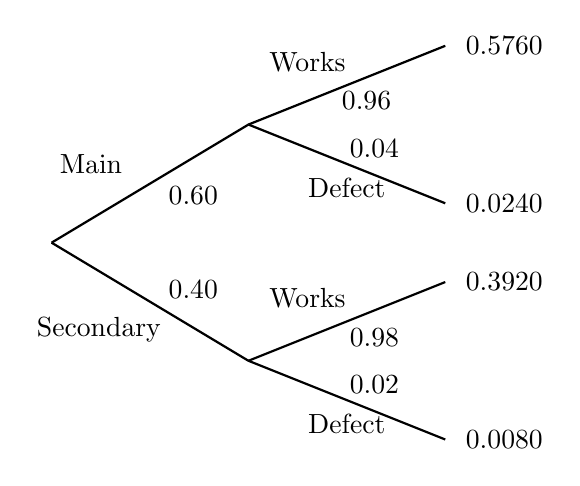
\begin{tikzpicture}[scale= 1.0]
		\def\FirstUpLabel{Main}
		\def\FirstDownLabel{Secondary}
		\def\SecondUpLabel{Works}
		\def\SecondDownLabel{Defect}
		\def\Up{$0.60$}
		\def\Down{$0.40$}
		\def\UpUp{$0.96$}
		\def\UpDown{$0.04$}
		\def\DownUp{$0.98$}
		\def\DownDown{$0.02$}
		\def\first{$0.5760$}
		\def\second{$0.0240$}
		\def\third{$0.3920$}
		\def\fourth{$0.0080$}
		
		\node at (0.5,1) {\FirstUpLabel};	
		\node at (0.6,-1.1) {\FirstDownLabel};	
		\node at (1.8,0.6) {\Up};
		\node at (1.8,-0.6) {\Down};
		\draw[thick] (0,0) -- (2.5,1.5);
		\draw[thick] (0,0) -- (2.5,-1.5);
		
		\node at (3.25,2.3) {\SecondUpLabel};
		\node at (3.75,0.7) {\SecondDownLabel};
		\node at (4,1.8) {\UpUp};
		\node at (4.1,1.2) {\UpDown};
		\node at (5.75,2.5) {\first};
		\node at (5.75,0.5) {\second};
		\draw[thick] (2.5,1.5) -- (5,2.5);
		\draw[thick] (2.5,1.5) -- (5,0.5);

		\node at (3.25,-0.7) {\SecondUpLabel};
		\node at (3.75,-2.3) {\SecondDownLabel};
		\node at (4.1,-1.2) {\DownUp};
		\node at (4.1,-1.8) {\DownDown};
		\node at (5.75,-0.5) {\third};	
		\node at (5.75,-2.5) {\fourth};	
		\draw[thick] (2.5,-1.5) -- (5,-0.5);
		\draw[thick] (2.5,-1.5) -- (5,-2.5);
		\end{tikzpicture}
		\]


\end{document}